% !TeX root = ../../../main.tex
\section{高维手写数字序贯识别实验}\label{cw:sec:ml-experiments}

第~\ref{cw:sec:sim-logistic}~节在一维零过程噪声系统上表明，离散最优输运可通过相邻源粒子的分位数凸插值避免单点坍缩。为进一步检验观测空间跃升至高维且潜空间达到十余维时，基于似然权重的离散变换与无权重的连续条件输运映射（第~\ref{cw:sec:ml-transport-theory}~节与第~\ref{cw:sec:ml-updates}~节）各自的表现边界，本节在 MNIST 手写数字数据集\cite{lecun1998gradient}上开展逐窗口含噪序贯识别实验。

\subsection{实验设置与评价指标}

实验采用 MNIST 标准划分中的 $M=60000$ 幅训练图像（像素归一化至 $[0,1]$ 并展平为 $n_D=784$ 维向量）拟合网络与经验先验，取测试集前 $500$ 幅图像开展定量评估。潜空间维数设为 $n_d=16$，压缩算子 $\mathscr T_{\Rightarrow}$、还原算子 $\mathscr T_{\Leftarrow}$ 与类别读出映射 $\ell$ 均采用多层全连接网络实现；在无噪完整测试图像上直接执行压缩与读出（$\ell\circ\mathscr T_{\Rightarrow}$）的测试重构均方误差为 $0.0093$，分类准确率为 $97.8\%$，作为各序贯滤波方法的性能上限参照。序贯观测按式~\eqref{cw:eq:ml-model} 生成：局部窗口边长取 $r=7$，按自左向右、自上而下的无重叠顺序分 $K=16$ 步扫完全图，窗口观测噪声标准差取 $\sigma=0.3$，默认粒子规模为 $N=256$。

实验共对比五种潜空间更新方案：
（1）\textbf{BPF}：每步按式~\eqref{cw:eq:ml-weights} 计算似然权重并执行多项重采样；
（2）\textbf{BPF 加扰动}：在多项重采样后对潜空间粒子叠加强度为 $0.1$ 的各向同性正态扰动，作为缓解零过程噪声粒子贫化的启发式基线；
（3）\textbf{ETPF}：熵正则化强度取当步代价矩阵均值的 $0.005$ 倍，执行 $50$ 轮稳定化交替尺度缩放（Sinkhorn 迭代）；
（4）\textbf{逐步在线 OTPF}：依据文献\cite{aljarrah2024brenier} 的极大极小框架独立复现，每步在线执行 $300$ 轮外层迭代（检验网络每更新 $1$ 次，输运网络更新 $5$ 次），并将 $49$ 维窗口观测投影至前 $4$ 个主特征方向以稳定小样本对抗训练；为确保基线充分调优，ETPF 与逐步 OTPF 的关键超参数均在测试集前 $100$ 幅图像上网格择优固定；
（5）\textbf{静态摊销 OTPF}（算法~\ref{cw:alg:amortized-otpf}）：离线阶段以批量大小 $1024$、内层比例 $5:1$ 训练 $240\,\mathrm{s}$，在线阶段仅执行式~\eqref{cw:eq:ml-amortized-update} 的单次前向映射。

评估采用四项互补指标：（i）式~\eqref{cw:eq:ml-vote} 粒子众数判决的识别准确率；（ii）类别后验平方误差，定义为粒子读出类别经验频率向量与真实类别独热示性向量之差的平方二范数，用于精细衡量后验概率校准程度；（iii）还原均方误差，即等权后验粒子经还原算子解码所得均值图像与真实无噪图像的像素均方误差；（iv）每幅测试图像每个观测步的平均在线推理耗时（批量并行计时）。主实验固定网络参数，以 $3$ 个独立随机种子重复抽样初始先验粒子与观测噪声序列，汇报均值与样本标准差。

\subsection{主要实验结果与机制分析}

\begin{table}[!htb]
\centering
\caption{MNIST 逐窗口序贯数字识别主实验结果}
\label{cw:tab:ml-main}
\vspace{0.5em}\wuhao\setlength{\tabcolsep}{5pt}
\begin{tabular}{lccccc}
\toprule[1.5pt]
 & \multicolumn{2}{c}{识别准确率（\%）$\uparrow$} & 类别后验 & 还原 & 每步在线耗时 \\
方法 & $k=8$ & $k=16$ & 平方误差 $\downarrow$ & 均方误差 $\downarrow$ & （ms）$\downarrow$ \\
\midrule[1pt]
BPF & $49.1\pm3.0$ & $49.2\pm3.1$ & $1.016\pm0.062$ & $0.0762$ & $0.034$ \\
BPF 加扰动 & $51.1\pm1.5$ & $53.9\pm1.7$ & $0.802\pm0.030$ & $0.0527$ & $0.034$ \\
ETPF & $54.3\pm1.4$ & $54.7\pm1.0$ & $0.902\pm0.021$ & $0.0638$ & $0.24$ \\
逐步在线 OTPF & $66.3\pm1.2$ & $81.8\pm1.4$ & $0.286\pm0.023$ & $0.0296$ & $17.2$ \\
静态摊销 OTPF & $\mathbf{92.1}\pm0.9$ & $\mathbf{96.8}\pm0.2$ & $\mathbf{0.045}\pm0.002$ & $\mathbf{0.0124}$ & $\mathbf{0.015}$ \\
\bottomrule[1.5pt]
\end{tabular}
\par\vspace{3pt}
{\wuhao 注：取 $N=256$，$500$ 幅测试图像，$3$ 个随机种子的均值 $\pm$ 标准差；后三列均为全图扫完时刻（$k=16$）的统计值\par}
\end{table}

表~\ref{cw:tab:ml-main} 与图~\ref{cw:fig:ml-curves} 展示了五种方法随观测窗口逐步揭示的定量表现。可以观察到两类截然不同的演化形态：凡依赖似然权重的方法（BPF、BPF 加扰动与 ETPF）均在扫描过半（$k=8$，恰好覆盖图像上半部）前陷入停滞，此后即便下半幅数字笔画完整揭示，识别准确率亦几乎不再增长，末步全部停留在 $49.2\%$--$54.7\%$ 之间。其根源在于 $16$ 维潜空间中的稀疏采样与零过程噪声叠加：对 BPF 而言，前几步局部窗口似然已将不同祖先粒子数由 $256$ 迅速压缩至接近 $1$（图~\ref{cw:fig:ml-curves}（d）离散度归零），一旦锁死于某个仅与上半部笔画相似的错误类别粒子，后续观测便因支撑集单点化而丧失修正能力，直接印证了定理~\ref{cw:thm:bpf-impoverishment}。更值得注意的是，在第~\ref{cw:sec:sim-logistic}~节一维系统中表现优异的 ETPF 在此仅比 BPF 提高 $5.5$ 个百分点：在 $16$ 维空间中，$256$ 个初始粒子高度稀疏，当单步似然权重集中于一两个粒子时，式~\eqref{cw:eq:particle-ot-transform} 的凸组合重心同样收缩至该少数粒子邻域，无法跨越潜空间空白区域生成新的假设模式；人工添加各向同性正态扰动虽维持了表面离散度，但盲目扩散偏离了任务流形方向，同样难以恢复正确类别。

\begin{figure}[!htb]
\centering
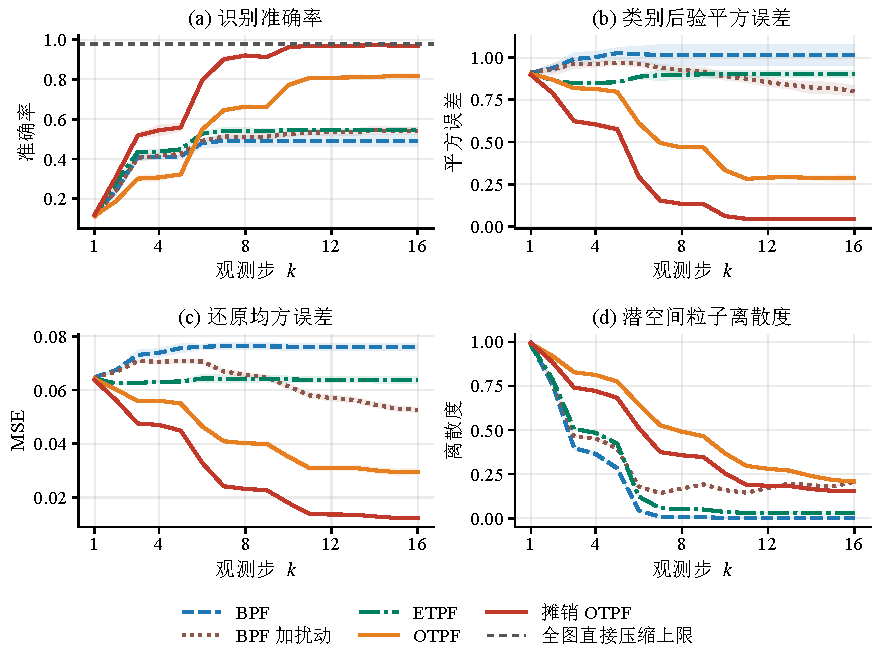
\includegraphics[width=0.94\linewidth]{figs/completed_work/ml_curves.pdf}
\par\vspace{3pt}
{\wuhao 注：实线/虚线为 $3$ 个随机种子的均值，浅色阴影为 $\pm1$ 倍标准差区间；图（a）水平灰虚线表示无噪全图直接压缩读出上限（$97.8\%$）\par\vspace{2pt}}
\caption{五种潜空间滤波方法的各项评价指标随观测步数的演化}
\label{cw:fig:ml-curves}
\end{figure}

\begin{figure}[!htb]
\centering
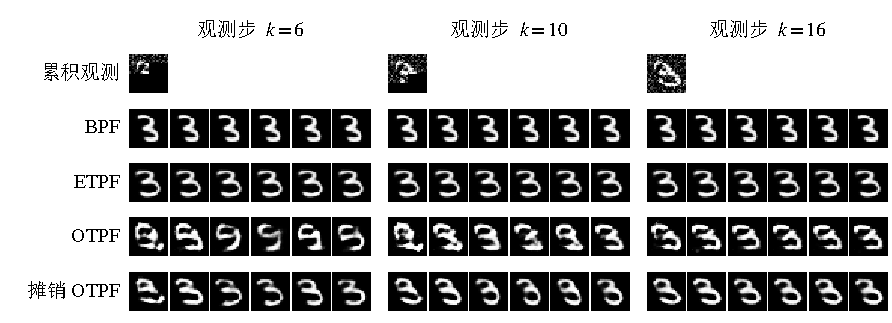
\includegraphics[width=0.96\linewidth]{figs/completed_work/ml_gallery.pdf}
\par\vspace{3pt}
{\wuhao 注：首行为 $k=6,10,16$ 时的含噪累积窗口观测（真实数字为 $3$），其余各行为对应时刻前 $6$ 个等权粒子的还原图像\par\vspace{2pt}}
\caption{单幅测试图像上四类方法的潜空间粒子解码演化对比}
\label{cw:fig:ml-gallery}
\end{figure}

相反，脱离似然权重的两类条件输运映射方法在整个扫描周期内随信息累积持续改善。逐步在线 OTPF 在末步达到 $81.8\%$ 的识别准确率，证明连续神经网络映射可将粒子主动推向任意潜空间区域；但由于每步仅凭 $N=256$ 个合成粒子对开展短期对抗训练，映射近似误差在 $16$ 次递推复合中不断累积，且单步在线训练使每图每步耗时高达 $17.2\,\mathrm{ms}$（约为 BPF 的 $506$ 倍）。静态摊销 OTPF 在半幅观测（$k=8$）时即达到 $92.1\%$，全图观测后达到 $96.8\%$，距无噪全图直接压缩上限（$97.8\%$）仅差 $1.0$ 个百分点，同时类别后验平方误差（$0.045$）与像素还原均方误差（$0.0124$）均显著低于所有对照方法；得益于在线阶段仅需一次前向张量运算，其每步推理耗时仅为 $0.015\,\mathrm{ms}$，比逐步在线 OTPF 快三个数量级。图~\ref{cw:fig:ml-gallery} 直观印证了上述差异：面对真实类别为“$3$”的测试图像，BPF 与 ETPF 在 $k=6$ 时 $6$ 个粒子已完全坍缩为同一固定笔画；逐步 OTPF 保留了多样性但解码轮廓存在局部畸变；静态摊销 OTPF 在早期局部观测存在歧义（$k=6$）时保持“$2$”“$3$”等多种合理笔画假设，随中下部窗口陆续揭示（$k=10,16$）平滑收拢至清晰的真实数字形态。

\subsection{粒子规模与潜空间维数消融}

\begin{table}[!htb]
\centering
\caption{粒子规模 $N$ 对末步识别准确率（$k=16$）的影响}
\label{cw:tab:ml-particles}
\vspace{0.5em}\wuhao
\begin{tabular}{lcccc}
\toprule[1.5pt]
方法 & $N=64$ & $N=256$ & $N=1024$ & $N=4096$ \\
\midrule[1pt]
BPF & $33.2\%$ & $46.6\%$ & $61.0\%$ & $72.0\%$ \\
BPF 加扰动 & $32.6\%$ & $56.2\%$ & $67.2\%$ & $81.4\%$ \\
ETPF & $36.4\%$ & $54.2\%$ & $69.6\%$ & -- \\
静态摊销 OTPF & $\mathbf{96.6\%}$ & $\mathbf{96.8\%}$ & $\mathbf{97.2\%}$ & $\mathbf{97.4\%}$ \\
\bottomrule[1.5pt]
\end{tabular}
\par\vspace{3pt}
{\wuhao 注：单个随机种子评估结果；$N=4096$ 时 ETPF 因 $N\times N$ 耦合矩阵开销过大未予运行\par}
\end{table}

表~\ref{cw:tab:ml-particles} 考察粒子规模 $N\in\{64,256,1024,4096\}$ 对末步准确率的影响（逐步在线 OTPF 因大规模粒子在线训练耗时过高未纳入该组扫描）。三类依赖权重的方法随 $N$ 增大稳步提升，印证了加密初始先验覆盖能够缓解有限支撑漏失；但即便在 $N=4096$ 下，BPF（$72.0\%$）与加扰动基线（$81.4\%$）仍远低于静态摊销 OTPF 在 $N=64$ 时的精度（$96.6\%$）。同时，ETPF 的每步耗时由 $N=256$ 时的 $0.24\,\mathrm{ms}$ 跃升至 $N=1024$ 时的 $7.9\,\mathrm{ms}$（增长逾 $30$ 倍），凸显了 $O(N^2)$ 耦合矩阵缩放在中等粒子规模下的可扩展性瓶颈。静态摊销 OTPF 对粒子规模极不敏感：由于单次映射已直接近似真实条件后验 $\mathbb P_{Z_k\mid Y_{1:k}=y_{1:k}}$，众数分类只需稳健估计十个离散类别的后验概率质量，$N=64$ 个粒子已足以给出低方差判决。

\begin{table}[!htb]
\centering
\caption{潜空间维数 $n_d$ 对重构精度与末步识别准确率的影响}
\label{cw:tab:ml-dim}
\vspace{0.5em}\wuhao
\begin{tabular}{cccccc}
\toprule[1.5pt]
$n_d$ & 测试重构均方误差 $\downarrow$ & 全图直接读出上限 & BPF & ETPF & 静态摊销 OTPF \\
\midrule[1pt]
$8$ & $0.0153$ & $95.5\%$ & $50.4\%$ & $57.6\%$ & $\mathbf{93.6\%}$ \\
$16$ & $0.0093$ & $97.8\%$ & $46.6\%$ & $54.2\%$ & $\mathbf{96.8\%}$ \\
$32$ & $0.0075$ & $98.2\%$ & $47.0\%$ & $55.0\%$ & $\mathbf{96.2\%}$ \\
\bottomrule[1.5pt]
\end{tabular}
\par\vspace{3pt}
{\wuhao 注：取 $N=256$，$k=16$，单个随机种子；$n_d=8,32$ 下摊销网络离线训练预算为 $150\,\mathrm{s}$，$n_d=16$ 下为 $240\,\mathrm{s}$\par}
\end{table}

表~\ref{cw:tab:ml-dim} 进一步考察潜空间维数 $n_d\in\{8,16,32\}$ 的折中效应。随着 $n_d$ 增加，还原流形的表达能力增强，测试重构均方误差单调下降（$0.0153\to0.0075$），全图直接读出上限相应升至 $98.2\%$。与之相对，BPF 与 ETPF 在 $n_d=8$ 时反而略高于 $n_d=16,32$，反映了重要性采样随潜维数升高而加剧的权重退化趋势。静态摊销 OTPF 在三个维数下均稳定逼近各自的全图读出上限；$n_d=32$ 略低于 $n_d=16$（$96.2\%$ 对 $96.8\%$）主要源于补充消融采用了较短的固定离线训练时长（$150\,\mathrm{s}$ 对 $240\,\mathrm{s}$）且高维输运网络收敛略慢。总计计算成本方面，在表~\ref{cw:tab:sim-environment} 所示单张 GPU 环境下，完成主实验全部三个网络的离线训练及五种方法的在线评估共耗时 $426\,\mathrm{s}$（其中摊销映射离线训练占 $240\,\mathrm{s}$，逐步在线 OTPF 评估占 $152\,\mathrm{s}$），包含多种子重复与两项消融在内的完整实验流程总计耗时 $1118\,\mathrm{s}$。
